\section{Introducción}
\subsection{La semilla del internet}  
El telégrafo fue el antecesor del teléfono, un primer acercamiento a la comunicación de
mensajes vía una codificación. Desde fines de siglo XIX hasta segunda mitad del siglo XX,
aparecen las centrales de \textbf{conmutación de circuitos} (centrales telefónicas). A estas centrales
llegaban señales (cables) correspondientes a todas las casas que participacen en el sistema de
teléfonos. Las operadoras conectaban dos circuitos en sus tableros para cerrar el circuito y
permitir la comunicación entre las dos partes involucradas. Sin embargo, este tipo de comunicación tenía una gran falla: Si una central de conmutación de circuitos
dejaba de estar disponible por algún motivo de fuerza, todas las personas pertenecientes a esa
zona se verían incomunicadas.


A fines de los 50 se empieza a desarrollar la \textbf{conmutación de paquetes} buscando resolver este tema, es decir se busca una \textbf{red más tolerante a fallas}, \textbf{más flexible} a la hora de conectar dos puntos distantes y que \textbf{escale más facilmente} ante un incremento en el acceso a la comunicación.

La nueva red propuesta es una red descentralizada con mútiples caminos entre dos puntos que divide los paquetes en fragmentos que pueden llegar a destino a través de distintos caminos.

\subsection*{El modelo OSI}
En 1983 aparece una publicación de ISO para establecer un estándar que especifique la estructura de una arquitectura de red, que uniformice la forma de construir las redes de cominucación: el modelo OSI-ISO (Open Systems Interconnection).

\begin{figure}[h]
	\centering
	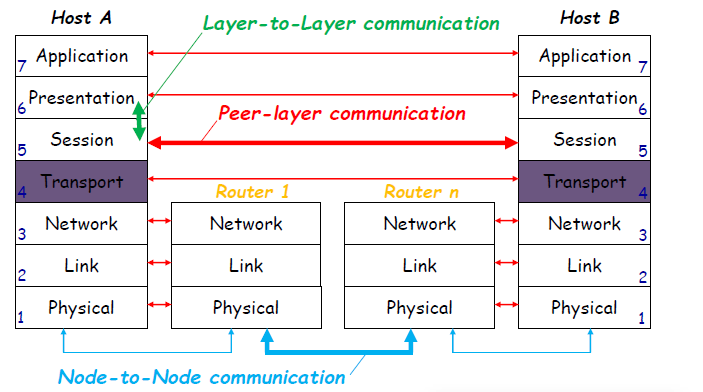
\includegraphics[width=0.65\textwidth
]{images/osi.png}
	\caption[Modelo OSI de Referencia]{Modelo OSI}
	\label{fig:osi}
\end{figure}

Este modelo está dividido en 7 capas, cada una de las cuales tiene una función definida que permitirán la comunicación coherente entre dos sistemas remotos.  

\begin{enumerate}
  \item La capa \textbf{física (Physical)} se encarga de enviar raw bits a través de los medios físicos disponibles en la red. 
  \item La capa de \textbf{enlace (Link)} se encarga de detectar errores en la transmisión y corregirlos, si es posible.
  \item La capa de \textbf{red (Network)} se encarga de resolver problemas de congestión dentro de la red, que paquetes se aceptan y la ruta que deben tomar los paquetes que se envían por la misma.
  \item La capa de \textbf{transporte (Transport)} se encarga de tomar la información provista por la capa de arriba, pasarla a la capa de red separada en pedazos más chicos (\textbf{chunks}) y se asegura que todas las partes lleguen a destino correctamente. 
  
  Esta es la primer capa \textbf{end-to-end}, es decir que entabla una "conversación" entre la máquina emisora (\textbf{Source}) y la destinataria (\textbf{Destination}). Las capas anteriores, usan protocolos de comunicación nodo a nodo, es decir, entre una máquina y su vecino inmediato y no entre el source y el destination que podrían estar separados entre sí por varios nodos.
  
  \item La capa de \textbf{sesión  (Session)} permite establecer sesiones entre dos máquinas distintas. Estas sesiones permiten sincronizar el pasaje de información entre ambas máquinas, deciden de quien es el turno para enviar información y evitar que ambas máquinas realizen operaciones críticas de manera simultanea.
  \item La capa de \textbf{presentación (Presentation)} procesa la información recibida, la estructura y la codifica de la manera necesaria para que pueda ser usada por la máquina.
  \item La capa de \textbf{aplicaciones (Application)} contiene los protocolos necesarios para que los usuarios puedan ver y leer la información.
\end{enumerate}

Además de estas funcionalidades, cada capa ofrece una interfaz que le permite comunicarse con las capas vecinas para hacer el pasaje de los datos entre ellas y asumen que el host en el otro extremo de la comunicación tendrá una arquitectura similar y podrá interpretar los mensajes de cada una de ellas.

\subsection{Modelo TCP/IP}
\begin{figure}[H]
	\centering
	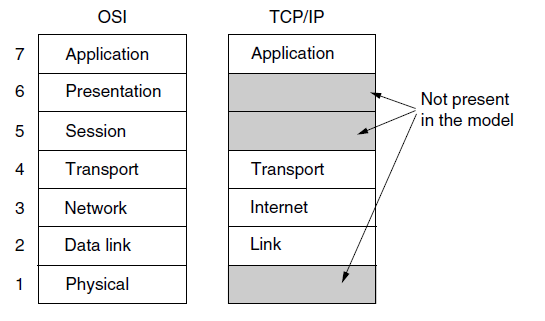
\includegraphics[width=0.65\textwidth
]{images/tcpip.png}
	\caption[Modelo TCP/IP de Referencia]{Modelo TCP/IP}
	\label{fig:tcp}
\end{figure}

Fue diseñado con el objetivo de mantener las conexiones intactas mientras ambos puntos finales de conexión estén funcionando, incluso si laguno de las máquinas o líneas entre ellos fuese dado de baja.

\begin{enumerate}
  \item La capa de \textbf{enlace (Link)} describe que deben cumplir los enlaces (cable de ethernet, lineas telefónicas, etc) para poder usados como medios de trasporte para este tipo de conexión.
  \item La capa de \textbf{intrared (internet)} permite al host injectar paquetes en cualquier red y se encarga de hacerlos llegar a destino. Esto se hacer de manera independiente para cada paquete, es decir pueden no seguir el mismo camino e incluso podrían llegar en distinto orden. En el último caso corresponde a la capas superiores reodenarlos para que puedan ser procesados, si es necesario.
  \item La capa de \textbf{transporte (Transport)} debe ser diseñada para permitir que dos entidades de la red puedan mantener una conversación. Aquí se definieron dos protocolos:
  \begin{itemize}
    \item El \textbf{Transmission Control Protocol (TCP)} que permite enviar sin errores un stream de bytes desde una máquina a otra en la red.
    \item El \textbf{User Datagram Protocol (UDP)} que permite evitar todo el flujo de conexión TCP y crear el suyo propio. En general, se usa en aplicaciones que requieren una respuesta más rápida que precisa. 
  \end{itemize}
  \item La capa de \textbf{Aplicación (Application)} que se incluye la sesiones y funciones necesarias para codificar y procesar los paquetes enviados y recibidos. Entre los protocolos usados en esta capa se encuentran: TELNEt, FTP y SMTP.
\end{enumerate}
